\chapter{Working of Tool}
\label{ch:work}
An ethereum smart contract after compilation generates bytecode. This byecode is deployed on the ethereum blockchain. The source code is not stored on blockchain. Hence there is no way to know the source code of a deployed smart contract. Etherscan\cite{etherscan} is a Block Explorer, Search, API and Analytics Platform for Ethereum. Among other things they also provide the source code verification as a service. Anyone can use this service to attach a source code with any deployed smart contract. The tool build the deployment payload and check if the same payload is on blockchain or not. If both matches then the source code is linked to the payload on etherscan\cite{ptb}. Hence we can find source code of many smart contracts on etherscan. Since there are millions of smart contracts deployed on blockchain not all smart contract's source code can be found on etherscan. But for the working of our tool we only need bytecode of smart contract instead of source code. The bytecode of a smart contract is given as input to the Tool, it processes the bytecode and generates the output as shown in the figure below.\\
\begin{center}
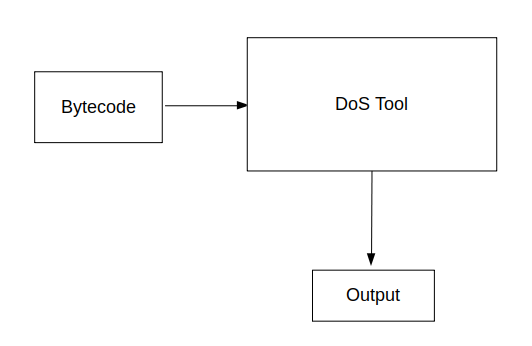
\includegraphics[width = 12cm, height = 7cm]{images/1.png}

    Figure 1
\end{center}
The output of the Tool will print the respective vulnerabilities as discussed under the topic Vulnerabilities Patterns in chapter 4.
\section{Insight of Components of Tool}
We will now dive deep into DoS Tool working. The bytecode is feed to the \textbf{\emph{parser}} which prepossess the bytecode. The \textbf{\emph{parser}} converts bytecode into opcode view named as parsed code in the tool. These opcodes and the control flow graph are feed to the \textbf{\emph{Symbolic Execution Phase}} which is the Custom EVM executed symbolically. The Symbolic Execution Phase along with the output also update a list of visited nodes. These list of visited nodes are the nodes that can be visited during the execution of Symbolic Execution. Hence these list of nodes are a subset of the nodes present in the Static CFG.\\ 
\begin{center}
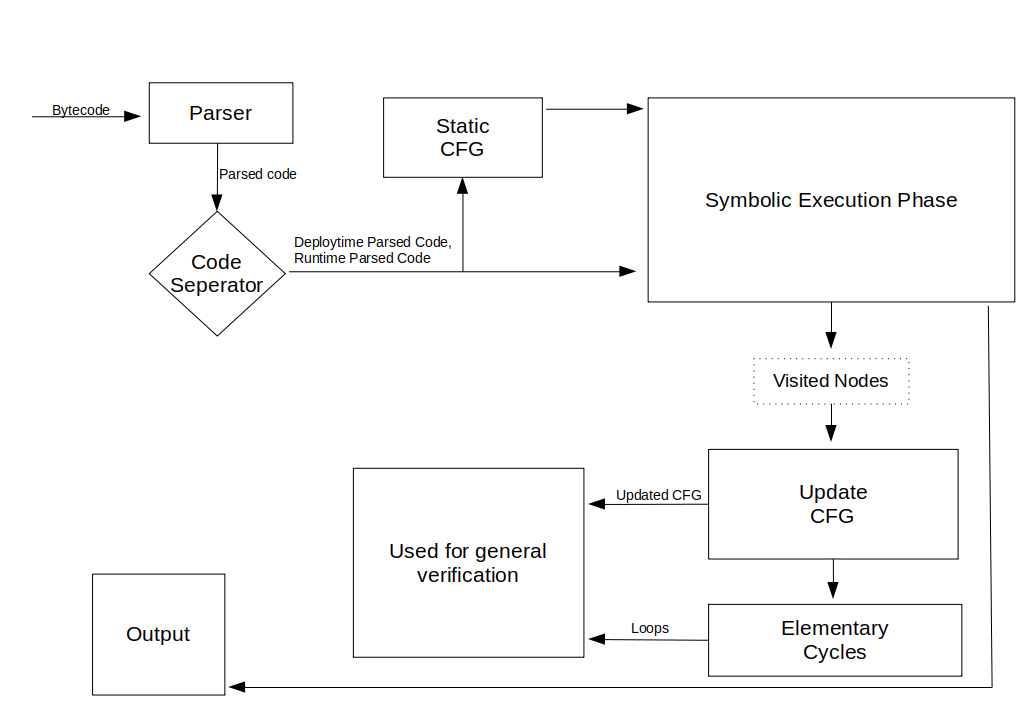
\includegraphics[width = 14cm, height = 12cm]{images/2.png}
Figure 2 : Components of Tool
\end{center}
The \textbf{\emph{Symbolic Execution Phase}} also resolves new paths which were not able to be resolved statically. This path resolution will be discussed in detail. Using the visited node list we update the Static CFG by deleting the nodes from the CFG which are not present in the visited node list. The graph algorithms to find elementary cycles are used to find loops in the updated CFG.The \emph{Updated CFG} is used to find the number of paths that can be traversed. The numbers in most cases should not match with the number of paths found in Static CFG because of overestimation of paths. This will be discussed in the subsequent topics. A flow diagram of the DoS Tool is shown in the Figure 2.


\noindent Let's discuss the Components of Tool in detail.
\subsection{Parser}
Bytecode is hexadecimal representation of the smart contract\cite{bytecode}. EVM(Ethereum Virtual Machine) has predefined opcodes. EVM understand these opcodes. The hexademicals in the bytecode corresponds to these opcodes. For example, \textbf{PUSH1} is an opcode which pushes 1 byte of the data on the stack. The corresponding hexadecimal value is \textbf{'0x60'}. Similarly \textbf{MSTORE} is an opcode which stores data in memory. The corresponding opcode is \textbf{'ox52'} and many more. The size of every opcode is 1 byte. Data in the bytecode can have a maximum of 32 bytes size. PUSH is an opcode which pushes constant data onto the stack without any computation. Hence such data is given directly in the bytecode in the hexadecimal format right next to the PUSH opcode. For example, the string \textbf{\emph{'6040'}} means \textbf{\emph{60}} corresponds to the PUSH1 opcode where 1 means 1 byte, hence PUSH1 pushes 1 byte of data on the stack. The next one byte, i.e., \textbf{\emph{40}} is the data which PUSH1 will push to the stack. We can find list of EVM opcodes and their corresponding hexadecimal value along with some extra information, such as, gas consumption of the opcode in the Ethereum Yellow Paper\cite{ethyellow} and also here\cite{ethop}.\\
The parser takes input the hexadecimal string(bytecode) and returns a list of these opcodes.
The list which parser returns have 4 fields.
\begin{itemize}
    \item \textbf{\emph{step}}: step corresponds to the position in the bytecode string. step is calculated in bytes. for example, let's consider the string '604052'. Here step = 0 means at 0th position in the string. step 1 corresponds to 2nd position in the string and so on. step can be used in the \textbf{JUMP/JUMPI} as an argument of position to jump to.
    \item \textbf{\emph{operand}}: operand is nothing but the hexadecimal value in the bytecode coresponding to the opcode. For example, in the string '604052', 60 is the operand for the opcode PUSH1.
    \item \textbf{\emph{input}}: input is the integer value of the corresponding hexademical data in the bytecode. For example, in the string '604052', the PUSH1(60) needs an input of 1 byte which will be right next to it, i.e., 40 in the string and its integer value is 64.
    \item \textbf{\emph{o}}: o is the opcode corresponding to hexadecimal value of the opcode in the bytecode. For example, in the string '604052', opcode corresponding to '60' is PUSH1 and opcode corresponding to '52' is MSTORE.
    
\end{itemize}
\noindent A sample parsed code of an opcode looks like below:
\begin{center}
    \textbf{\emph{\{'step' : 2, 'operand' : 60, 'input' : 64, 'o' : PUSH1\}}}
\end{center} 
step equals to 0 means the positions of this opcode is the 2nd byte in the bytecode, operand value at 2nd byte is 60, the input for the operand 60 is 64 and the opcode corresponding to the operand 60 is PUSH1. Hence parser converts bytecode into the custom opcode/assembly code list which we called as parsed code.
\subsection{Code Separator}
The bytecode is a combination of creation bytecode, we named it as deploytime bytecode and runtime bytecode, we named it as runtime bytecode. The runtime bytecode is the code that is stored on-chain that describes the smart contract. The deploytime bytecode generates the runtime bytecode, it includes constructor logic and constructor parameters. It is equivalent to the input data of the transaction which create smart contract\cite{diffop}. We have separated deploytime parsed code and runtime parsed code from the parsed code beforehand to feed to the other components of the DoS Tool. A static pattern search is performed to separate these two codes from the bytecode. \textbf{CODECOPY} is an opcode which is used to copy constructor parameters and to copy the runtime bytecode to the memory of the EVM. Also every bytecode, be it deploytime or runtime, starts with fixed instructions. These fixed instruction sets a pointer to the free memory pointer from where the program starts storing data in memory. These instructions are as follows
\begin{center}
    PUSH1 mm\\
    PUSH1 dd\\
    MSTORE
\end{center}
Here mm and dd are the hexadecimal 1 byte data for the PUSH1 opcodes. MSTORE needs two inputs the memory location where we want to store, i.e., mm and the data to store at the memory location, i.e., dd. Hence every deploytime bytecode or runtime btecode starts with a string '60mm60dd52'. The algorithm to separate bytcode is as follows.
\begin{Verbatim}[numbers=left,xleftmargin=5mm]
    Search for CODECOPY in the parsed code
    if CODECOPY found
    
        search for RETURN ahead
        if RETURN found
        
            search for the string ahead
            if CODECOPY found
                goto line 2
            if string found
                the parsed code above this position is deploytime bytecode
                the parsed code below from this position is runtime bytecode
                return
            if string NOT found
                return can't separate
                
        if CODECOPY found 
            goto line 2
        if RETURN not found
            return can't separate
            
    if CODECOPY not found
        return can't separate
\end{Verbatim}
\subsection{Static Control Flow Graph}
There is an opcode \textbf{JUMPDEST} in the EVM opcode list. The sole purpose of the opcode is to mark the beginning of a block. Every block starts with \textbf{JUMPDEST} except the very first block which starts with the magic string '60mm60dd52' as discussed under code separator component. Hence we can obtain list of basic blocks in the parsed code. Now these basic blocks needs to be connected in order to determine the control flow of the program. There are four ways to determine control flow of the program.
\begin{itemize}
    \item \textbf{JUMP} opcode: This is an unconditional jump. JUMP only takes one argument which is the destination of the jump. If the destination opcode is JUMPDEST then it is a valid jump else EVM stop traversing this path. When EVM encounters JUMP instruction it takes the current top value of the stack as argument and jumps to this location in the bytecode. This location argument is either directly pushed before JUMP instruction by using PUSH opcode or is a result of some computation, example - add, mul etc. Since we are not executing Custom EVM since, we don't have stack trace and we can only resolve the JUMP location only when its argument is directly pushed by PUSH instruction in the bytecode just before the JUMP instruction.
    \item \textbf{JUMPI} opcode: JUMPI is an conditional jump. JUMPI takes two argument, the top of stack is the jump location and the next value on the stack is a boolean condition value. If condition value is 1 the code jumps to the location provided by jump location argument and if the condition value is 0 the code continue executing without jump. Also if condition value is 1, the jump location in the bytecode is only valid if it is JUMPDEST opcode. JUMPI location can also remain unresolved like the JUMP location.
    \item \textbf{JUMPDEST} opcode: If on executing the current block JUMPDEST instruction is encountered, this is the starting of the next block and control is flowing directly from the current block to the next block. Therefore we simply connects the block with the next adjacent block.
    \item \textbf{INVALID}: If we encounter an INVALID opcode on traversing a block then it is the end of the block and this block is the end block in the path and not connected to any other block  in the control flow of the program.
\end{itemize}
The output of this component is a control flow graph we named as STATIC CFG. The name static is added just to clarify that the control flow of the program is not obtained by executing the program and keeping track of the state trace of the program. There are two shortcomings to the CFG as discussed below.
\begin{itemize}
    \item \textbf{Overestimation of Paths}\\
    To determine static CFG no dynamic or symbolic approach is used. Hence the control flow paths are overestimated because we have considered all paths. There may be possibility that some paths will never be traversed for any inputs during the execution life of the program.
    \item \textbf{Unresolved JUMP/JUMPI}\\
    Even though the Static CFG is overestimated, the CFG may have missed the control flow that is possible to reach during the execution life of the program. This is mainly due to the reason of unresolved JUMP/JUMPI instructions as discussed above.
\end{itemize}
\subsection{Symbolic Execution Phase}
The Symbolic Execution Phase will run the bytecode in a Custom EVM symbolically. A diagram of Symbolic Execution Phase is shown in the Figure 3 below.\\
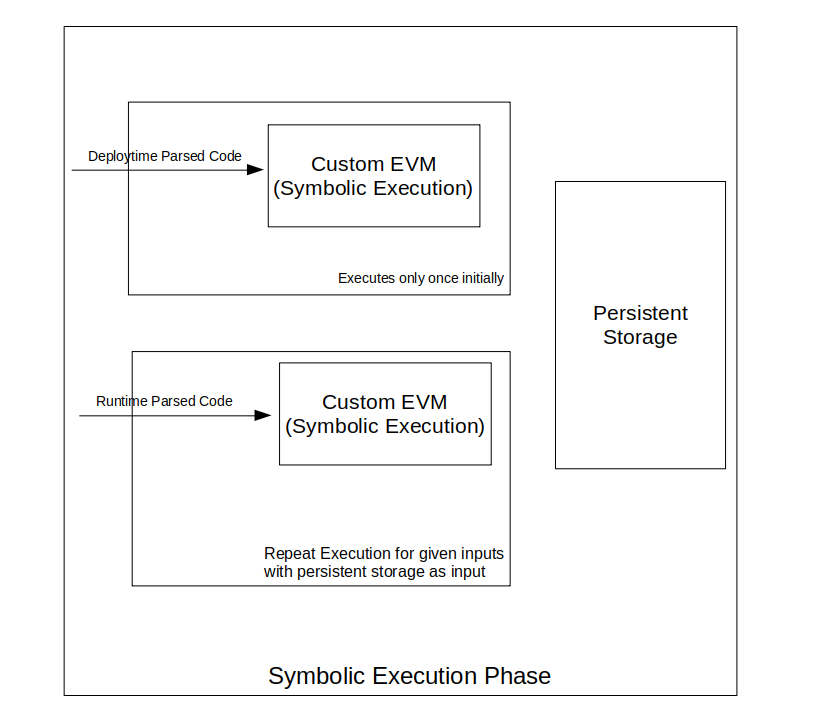
\includegraphics[width = 15cm, height = 14cm]{images/3.png}
\begin{center}
    Figure 3
\end{center}
EVM works on the bytecode of the smart contract. EVM is a stack based machine with the maximum limit of the stack is 1024. The EVM generally uses stack for intermediate values in computations. EVM also uses memory and storage other than stack. The memory is the real workhorse and is non-permanent. Storage is used for values which needs to be persists between different executions of the smart contract. Hence storage is permanent. The gas usage of storage is very high as compared to the memory. Hence one should wisely decide between what to store permanently and what should be temporary during smart contract execution. EVM also keeps track of the gas usage in order to terminate program when out of gas. The Custom EVM used in the Symbolic Analysis Phase implements the stack, memory and the storage, basically the state implementation. The Custom EVM don't implement other features of EVM. The idea for the implementation of custom EVM is taken from the tool Maian\cite{10.1145/3274694.3274743}\cite{maian}.\\
The Custom EVM starts executing the parsed code from the start. Any value which can be decided by external user is considered as symbolic. For example, CALLDATA of functions which can be called in order to interact with the smart contracts, the return value from the external smart contracts which were called from the contract, CALLVALUE - the value of ether send to a payable function by the external user. Upon traversing the exectuion path, these symbolic variables build symbolic expressions. When the control flow branches we use SMT solver to decide whether the further path is feasible of not. If the SMT solver returns not satisfiable for the certain path condition then it will not be traversed. We have taken few design choices in order to mitigate some of the problems as discussed below. 
\begin{itemize}
    \item \textbf{Infinite Loops}: Infinite loop detection is undecidable. Therefore during the execution of the Custom EVM, there may be possibility that the execution never stops. Hence we introduced maximum path length from the start of the execution. When the execution arrives at the new block the path length increases by one and if a certain path length reaches maximum path length limit the Custom EVM reverts and stops traversing the path. There is no way to decide what should be the appropriate value of maximum path length. Hence we tested the tool on three maximum path length, i.e, 10, 20 and 40. The maximum path length is given as input to the tool by the user.
    \item \textbf{Multiple Invocation of smart contracts}: Let's understand this with an example.
    \begin{Verbatim}[numbers=left,xleftmargin=5mm]
    pragma solidity ^0.4.24;
    contract BasicToken {
        uint256[] balances;
        function balanceOf() public  view returns (uint256) {
            uint c = 1;
            balances.push(a);
            return c;
        }
        function print() public view returns (uint256){
            uint256 temp = 0;
            for(uint256 i = 0; i < balances.length; i++){
                temp += balances[i];
            }
        return temp;
        }
    }
    \end{Verbatim}
    It is necessary to know how bytecode calls external function. The first 4 bytes of the keccak of the external function known as function signature are the identifier of functions in the bytecode.
    for example the function signature of \emph{print()} function in the above code will be '13bdfacd' and function signature of \emph{balanceOf()} function in the the code will be '722713f7'. The assembly view of external functions in the smart contract above is
    \begin{Verbatim}[numbers=left,xleftmargin=5mm]
        PUSH4 0x13BDFACD 
	EQ 
	PUSH2 0x51 
	JUMPI 
	DUP1 
	PUSH4 0x722713F7 
	EQ 
	PUSH2 0x7C 
	JUMPI
    \end{Verbatim}
    Hence the first for byte of the CALLDATA will be compared with the function signature and jump to the corresponding function block. Since our Custom EVM starts executing bytecode from the start, first the \emph{print()} function will be executed and then the \emph{balanceOf()} function. The loop condition in the \emph{print()} function is symbolic because of the \emph{balanceOf()} function. Hence balances.length will be set to symbolic when the Custom EVM executes \emph{balanceOf()} function. Therefore in the first invocation of the smart contract the vulnerability will not be captured. But since the balances.length is stored in the storage and we know storage is persistent, in the second invocation of the smart contract, even on executing the \emph{print()} function first again, the vulnerability will be captured because the balances.length was set to symbolic in the previous invocation of the CUstom EVM. Hence the tool should test on multiple invocations of the smart contract in order to capture such vulnerabilites. We have test on invocations 1 and 2 but this is also given as argument to the Custom EVM.\\
    \\
    \item \textbf{Constant Loops with iterations more than MAXIMUM PATH LENGTH}\\
    In constant loop the loop condition is constant and hence SMT solver can do nothing much but will traverse the loop iteration until loop completes. Only after completion of loop the path after the loop in the program will be traversed. Hence he branch of execution after a constant loop is only accessible after the completion of loop. Hence if a constant loop is terminated in between the path after the loop will never be traversed. Although we have made this design choice by keeping in mind that all paths will not be traversed for the cost of not trapping into the infinite loop. But we can break this constant loop early and since we know that loop condition is constant we can traverse the path after the loop instead of looping the maximum path length into the constant loop.
    This should also be noticed that these constant loops can also exceeds the block gas limit. So only constant loops for 10000 iterations are considered for our Custom EVM. EVM block gas limit in practice exceeds for loops around 2-4 lakhs of iterations. Again this can be set and not fixed in the Custom EVM.
\end{itemize}
Th Static CFG is also an input to the Symbolic Execution Phase to resolve the unresolved control flow paths as discussed in the Static CFG. We have also maintained a list of visited nodes. Whenever a new block is reached at any point in the exectution, on any invocation we add it to the visited list. Hence visited node is a list of blocks ever visited during the Symbolic Execution phase of the Tool.
\subsection{OUTPUT}
The symbolic Execution Phase outputs the vulnerability of the smart contract from the four vulnerabilities as discussed above and as safe if no vulnerability is found.
\subsection{Update CFG and Elementary Loops}
The updated CFG will used the visited nodes list updated by Symbolic Execution Phase as input. Update CFG will remove nodes and their paths from the Static CFG. Hence the number of paths in updated CFG are subsets of the path in the Static CFG. The number of paths corresponding to the Static CFG and Updated CFG are shown in the output of the Tool.\\
The elementary loops will find all the elementary loops in the updated CFG. It is to be noted that the loops found during the symbolic analysis phase are different from the loops obtained from the Updated CFG. After careful observation we noticed that the loops obtained during Symbolic Execution should be subset of the loops obtained from the Static CFG. There may be many reasons for this and we will see on reason with the help of Graph 1. Let the contract execution starts from node A and we will consider only 1 invocation of the smart contract. Suppose the control flow AC is not symbolically feasible during the execution of the smart contract. The execution can traverses path AB or ABC or ABCD or ABCDA. If we the execution goes all the way back to the A by traversing path ABCDA, then all the nodes will be in the visited nodes list. Hence the Static CFG and the Updated CFG will be same because we considered all visited nodes without considering whether the path from one node to another is actually feasible or not.\\
\begin{center}
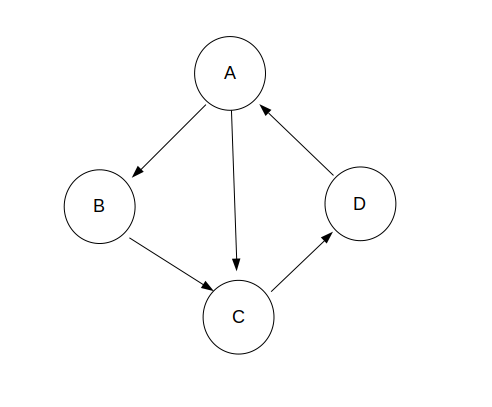
\includegraphics[width=10cm, height=7cm]{images/4.png}.

    Graph 1
\end{center}
Hence when we find loops using graph algorithm on the Updated CFG, we will get two loops ABCDA and ACDA, while the Symbolic Analysis Phase returns only 1 loop, i.e., ABCDA. These features are not necessary for the tools but we build these components in order to do some reasoning about the Tool.
